\documentclass[aspectratio=169,10pt]{beamer}

\usetheme{default}
\usepackage[T1]{fontenc}
\usepackage[utf8]{inputenc}
\usepackage{booktabs}
\usepackage{array}
\usepackage{tabularx}
\usepackage{tikz}
\usepackage{pgfplots}
\usepackage{xcolor}
\usepackage{amsmath}
\usepackage{ragged2e}
\usetikzlibrary{arrows.meta,positioning,fit,calc,shapes.geometric}
\pgfplotsset{compat=1.18}

\definecolor{Ink}{HTML}{06111F}
\definecolor{Panel}{HTML}{10263A}
\definecolor{PanelTwo}{HTML}{132F46}
\definecolor{Line}{HTML}{31506A}
\definecolor{Blue}{HTML}{2563EB}
\definecolor{Amber}{HTML}{F59E0B}
\definecolor{Cyan}{HTML}{38BDF8}
\definecolor{Green}{HTML}{22C55E}
\definecolor{Red}{HTML}{EF4444}
\definecolor{Muted}{HTML}{9CB4C8}
\definecolor{Paper}{HTML}{F8FAFC}

\setbeamercolor{normal text}{fg=Paper,bg=Ink}
\setbeamercolor{frametitle}{fg=Paper,bg=Ink}
\setbeamercolor{title}{fg=Paper,bg=Ink}
\setbeamercolor{progress bar}{fg=Amber,bg=Line}
\setbeamercolor{alerted text}{fg=Amber}
\setbeamercolor{block title}{fg=Paper,bg=PanelTwo}
\setbeamercolor{block body}{fg=Paper,bg=Panel}
\setbeamerfont{frametitle}{size=\Large,series=\bfseries}
\setbeamerfont{title}{size=\Huge,series=\bfseries}
\setbeamertemplate{itemize item}{\color{Amber}\small$\blacktriangleright$}
\setbeamertemplate{navigation symbols}{}
\setbeamertemplate{footline}{%
  \hfill\scriptsize\color{Muted}{Materials adversarial forensic review\hspace{1em}\insertframenumber/\inserttotalframenumber}\hspace{1em}\vspace{0.6em}}

\tikzset{
  box/.style={draw=#1, fill=Panel, rounded corners=2pt, very thick, align=center, text=Paper, inner sep=6pt},
  box/.default=Line,
  risk/.style={draw=Red, fill=Red!18!Ink, rounded corners=2pt, very thick, align=center, text=Paper, inner sep=6pt},
  good/.style={draw=Green, fill=Green!15!Ink, rounded corners=2pt, very thick, align=center, text=Paper, inner sep=6pt},
  warn/.style={draw=Amber, fill=Amber!15!Ink, rounded corners=2pt, very thick, align=center, text=Paper, inner sep=6pt},
  arrow/.style={-{Latex[length=2.5mm]}, very thick, draw=Muted},
  redarrow/.style={-{Latex[length=2.5mm]}, very thick, draw=Red}
}

\newcommand{\metric}[3]{%
  \begin{block}{#2}
  \centering{\Huge\bfseries\color{#3}#1}
  \end{block}
}

\title{Materials Adversarial Forensic Review}
\subtitle{Actual project evidence, generated architecture diagrams, and honest scientific claims}
\author{Materials Adversarial Learning Project}
\date{Generated from repository results}

\begin{document}

\maketitle

\begin{frame}{Executive Takeaway}
\begin{columns}[T,totalwidth=\textwidth]
\column{0.58\textwidth}
{\Large\bfseries The audit changes the story.}
\vspace{0.8em}

The model is genuinely unstable under token-level perturbations, but the original claim that \alert{length-changing perturbations cause the drift} does not survive forensic testing.

\vspace{1em}
\begin{block}{Defensible headline}
Real token-level instability exists; the length mechanism is refuted; chemistry-preserving robustness is not yet demonstrated.
\end{block}
\column{0.38\textwidth}
\metric{247}{Tg samples after cleaning}{Cyan}
\metric{$n=6$}{sealed test split}{Red}
\metric{86,337}{Transformer parameters}{Amber}
\end{columns}
\end{frame}

\section{Framing}

\begin{frame}{Problem Statement}
\begin{block}{Core problem}
Can polymer sequence models make stable property predictions under valid-looking PSMILES perturbations, or are observed adversarial effects artifacts of representation, data split, pooling, and attack design?
\end{block}

\begin{columns}[T,totalwidth=\textwidth]
\column{0.5\textwidth}
\begin{itemize}
  \item Sequence models can look accurate while learning syntax shortcuts.
  \item Token perturbations can change predictions without proving chemical vulnerability.
  \item Valid SMILES is not the same as a label-preserving material.
\end{itemize}
\column{0.46\textwidth}
\begin{itemize}
  \item The audit asks which claims survive.
  \item It separates model instability from causal mechanism.
  \item It identifies the experiments still needed before publication.
\end{itemize}
\end{columns}
\end{frame}

\begin{frame}{Research Questions}
\begin{enumerate}
  \item Are polymer sequence regressors vulnerable to valid token-space perturbations?
  \item Is the vulnerability specifically caused by length-changing edits?
  \item Does adversarial training generalize across attack families?
  \item Are current attack labels chemically justified as property-preserving?
  \item What exact gaps must be fixed before making a strong robustness claim?
\end{enumerate}
\end{frame}

\begin{frame}{Project Scope and Data}
\begin{columns}[T,totalwidth=\textwidth]
\column{0.52\textwidth}
\begin{block}{Tg forensic audit focus}
\begin{itemize}
  \item Raw table: 741 rows, 32 property columns.
  \item Tg non-null records: 443.
  \item RDKit canonicalization plus conflict dropping.
  \item Final Tg dataset: 247 samples.
  \item Scaffold split: 204 train / 37 validation / 6 test.
\end{itemize}
\end{block}
\column{0.44\textwidth}
\begin{block}{Older bandgap milestone}
\begin{itemize}
  \item 2,946 train / 631 validation / 632 test.
  \item Clean test MAE: 0.4619 eV.
  \item Test $R^2$: 0.8019.
\end{itemize}
\end{block}
\begin{alertblock}{Deck choice}
The Tg forensic audit is treated as the current headline because it supersedes the earlier length-mechanism narrative.
\end{alertblock}
\end{columns}
\end{frame}

\begin{frame}{Literature Gap}
\begin{itemize}
  \item Polymer property prediction often uses SMILES/PSMILES because strings are easy to tokenize.
  \item Transformer models can learn token context, but small polymer datasets make shortcut learning likely.
  \item Standard evaluations emphasize clean MAE and $R^2$ more than representation invariance.
  \item Adversarial chemistry work often blurs validity, plausibility, and unchanged target labels.
\end{itemize}

\vspace{0.8em}
\begin{block}{Exact gap this project exposes}
The missing control is a representation-level perturbation where the molecule and label are provably unchanged, plus matched-budget evaluation and cross-validated baselines.
\end{block}
\end{frame}

\section{Architecture}

\begin{frame}{Generated System Architecture}
\centering
\resizebox{0.98\textwidth}{!}{%
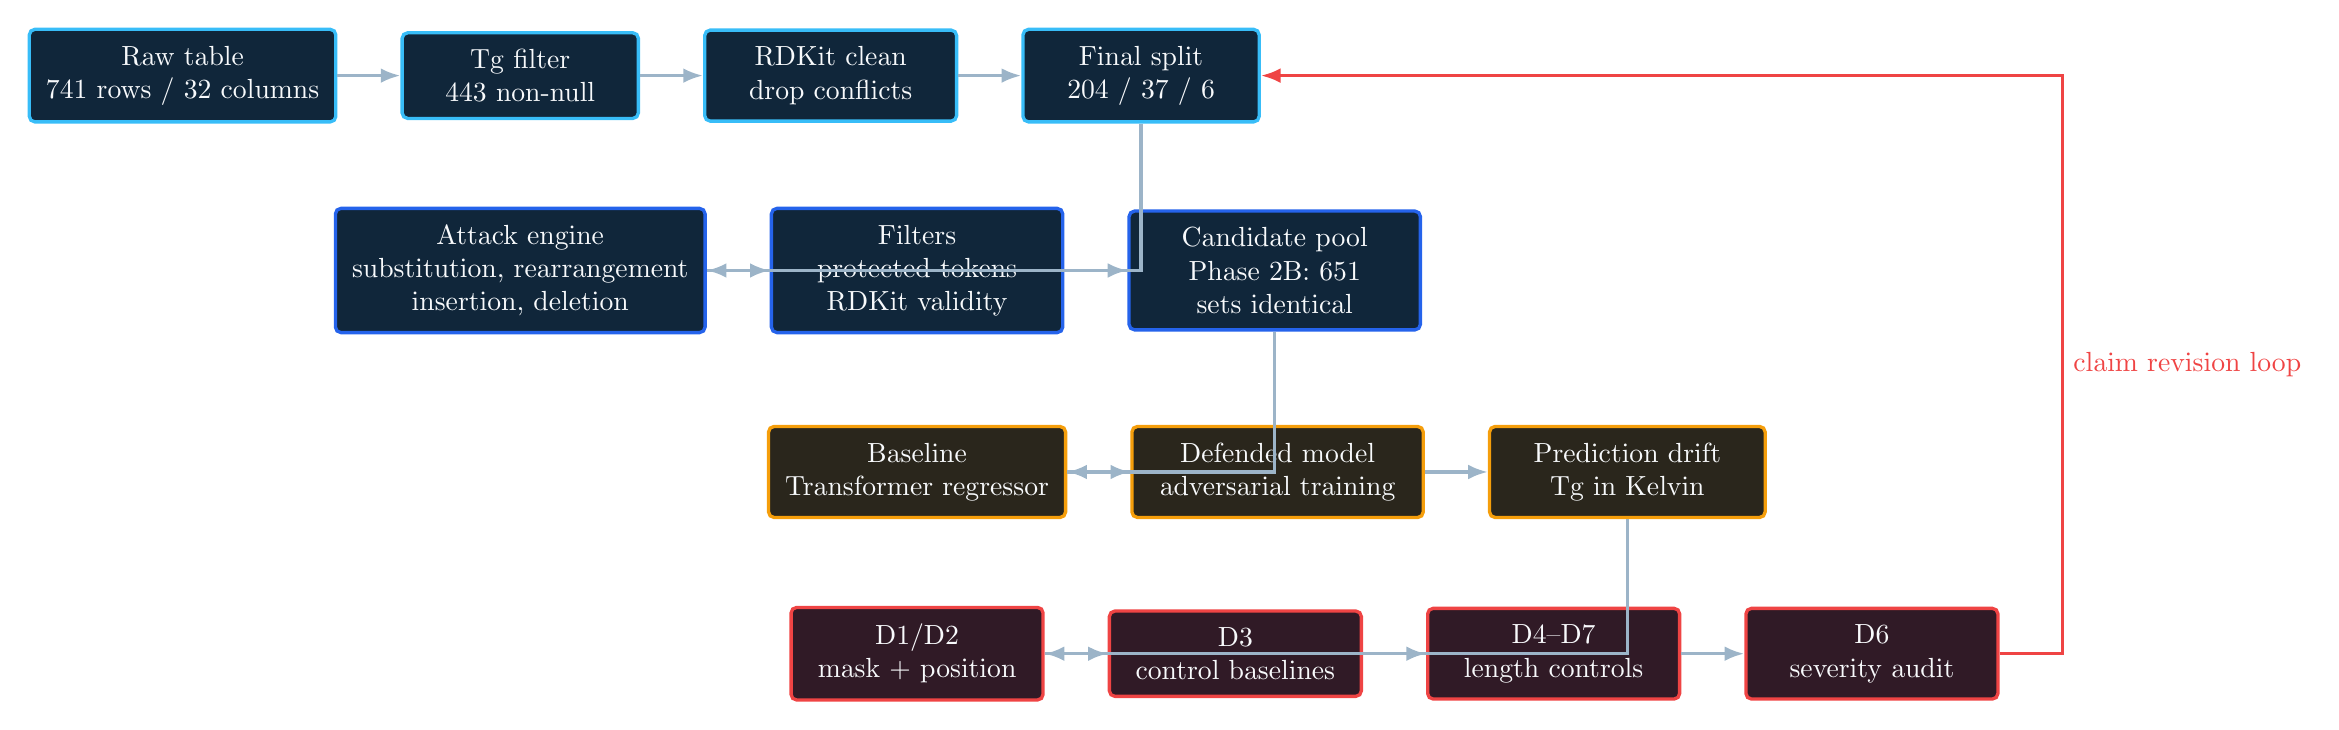
\begin{tikzpicture}[node distance=0.8cm]
  \node[box=Cyan, minimum width=3.0cm, minimum height=1.05cm] (raw) {Raw table\\741 rows / 32 columns};
  \node[box=Cyan, right=of raw, minimum width=3.0cm, minimum height=1.05cm] (filter) {Tg filter\\443 non-null};
  \node[box=Cyan, right=of filter, minimum width=3.2cm, minimum height=1.05cm] (clean) {RDKit clean\\drop conflicts};
  \node[box=Cyan, right=of clean, minimum width=3.0cm, minimum height=1.05cm] (split) {Final split\\204 / 37 / 6};
  \draw[arrow] (raw) -- (filter);
  \draw[arrow] (filter) -- (clean);
  \draw[arrow] (clean) -- (split);

  \node[box=Blue, below=1.1cm of filter, minimum width=4.0cm, minimum height=1.2cm] (attacks) {Attack engine\\substitution, rearrangement\\insertion, deletion};
  \node[box=Blue, right=of attacks, minimum width=3.7cm, minimum height=1.2cm] (valid) {Filters\\protected tokens\\RDKit validity};
  \node[box=Blue, right=of valid, minimum width=3.7cm, minimum height=1.2cm] (pool) {Candidate pool\\Phase 2B: 651\\sets identical};
  \draw[arrow] (split) |- (attacks);
  \draw[arrow] (attacks) -- (valid);
  \draw[arrow] (valid) -- (pool);

  \node[warn, below=1.15cm of valid, minimum width=3.7cm, minimum height=1.15cm] (base) {Baseline\\Transformer regressor};
  \node[warn, right=of base, minimum width=3.7cm, minimum height=1.15cm] (def) {Defended model\\adversarial training};
  \node[warn, right=of def, minimum width=3.5cm, minimum height=1.15cm] (pred) {Prediction drift\\Tg in Kelvin};
  \draw[arrow] (pool) |- (base);
  \draw[arrow] (base) -- (def);
  \draw[arrow] (def) -- (pred);

  \node[risk, below=1.1cm of base, minimum width=3.2cm, minimum height=1.05cm] (d1) {D1/D2\\mask + position};
  \node[risk, right=of d1, minimum width=3.2cm, minimum height=1.05cm] (d3) {D3\\control baselines};
  \node[risk, right=of d3, minimum width=3.2cm, minimum height=1.05cm] (d4) {D4--D7\\length controls};
  \node[risk, right=of d4, minimum width=3.2cm, minimum height=1.05cm] (d6) {D6\\severity audit};
  \draw[arrow] (pred) |- (d1);
  \draw[arrow] (d1) -- (d3);
  \draw[arrow] (d3) -- (d4);
  \draw[arrow] (d4) -- (d6);
  \draw[redarrow] (d6.east) -- ++(0.8,0) |- node[pos=0.25,right,text=Red] {claim revision loop} (split.east);
\end{tikzpicture}}
\end{frame}

\begin{frame}{Generated Model Architecture}
\centering
\resizebox{0.98\textwidth}{!}{%
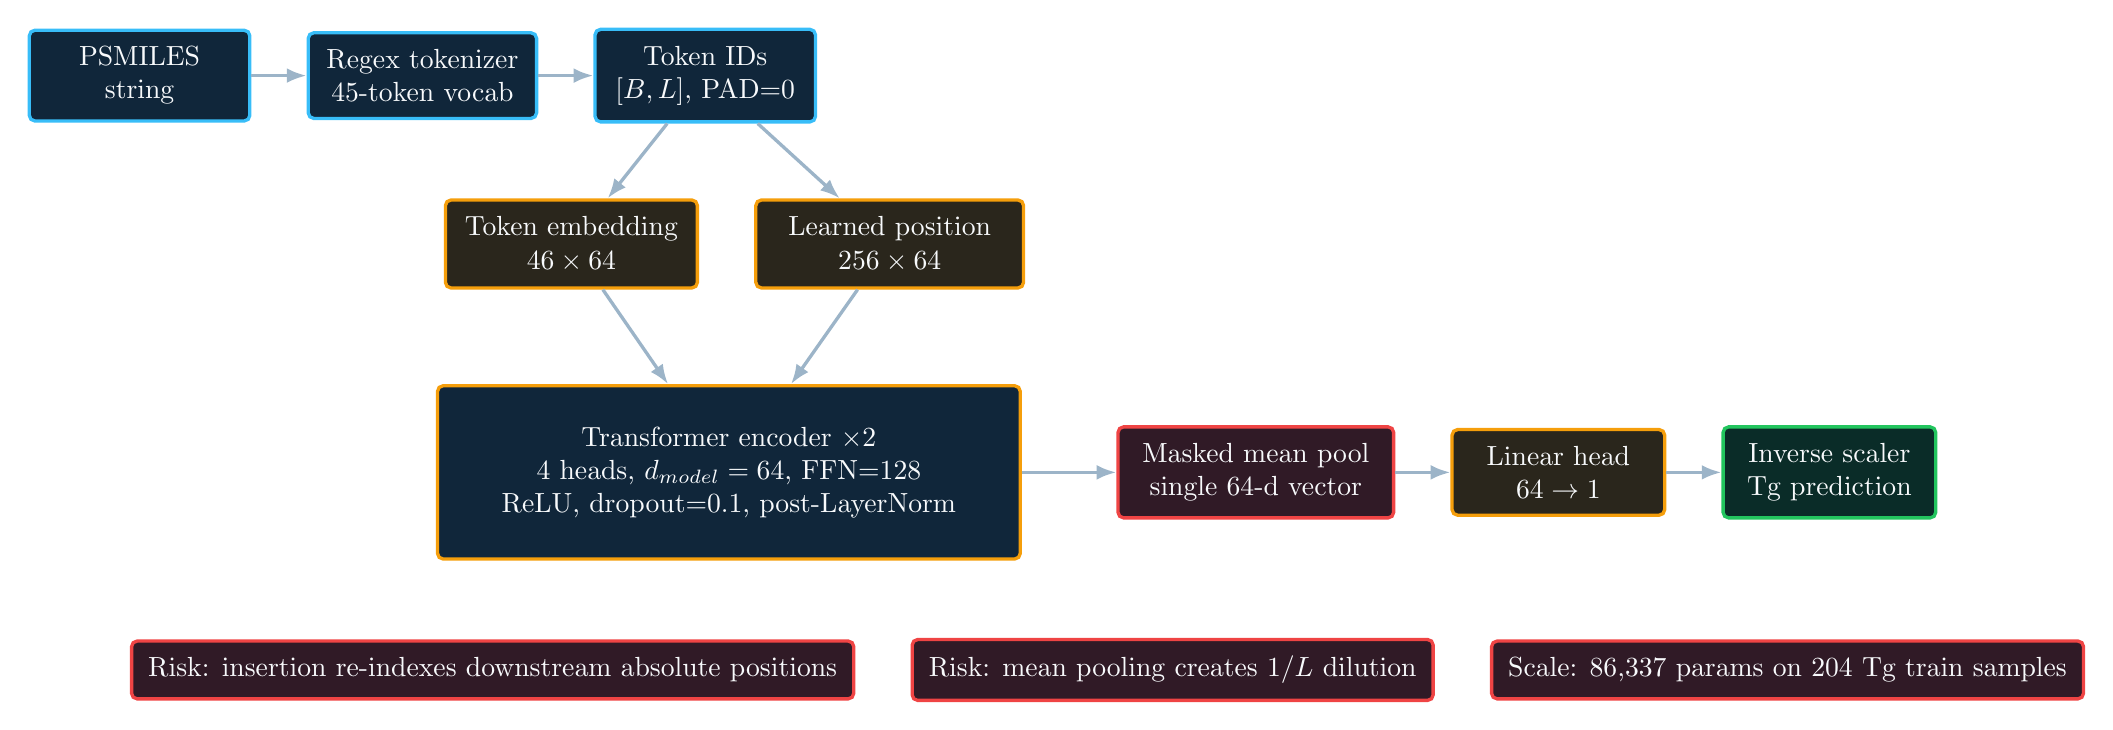
\begin{tikzpicture}[node distance=0.7cm]
  \node[box=Cyan, minimum width=2.8cm, minimum height=0.9cm] (ps) {PSMILES\\string};
  \node[box=Cyan, right=of ps, minimum width=2.9cm, minimum height=0.9cm] (tok) {Regex tokenizer\\45-token vocab};
  \node[box=Cyan, right=of tok, minimum width=2.8cm, minimum height=0.9cm] (ids) {Token IDs\\$[B,L]$, PAD=0};
  \draw[arrow] (ps) -- (tok);
  \draw[arrow] (tok) -- (ids);

  \node[warn, below=0.95cm of ids, xshift=-1.7cm, minimum width=3.2cm, minimum height=0.95cm] (te) {Token embedding\\$46 \times 64$};
  \node[warn, right=of te, minimum width=3.4cm, minimum height=0.95cm] (pe) {Learned position\\$256 \times 64$};
  \draw[arrow] (ids) -- (te);
  \draw[arrow] (ids) -- (pe);

  \node[box=Amber, below=1.2cm of te, xshift=2.0cm, minimum width=7.4cm, minimum height=2.2cm] (enc) {
    Transformer encoder $\times 2$\\
    4 heads, $d_{model}=64$, FFN=128\\
    ReLU, dropout=0.1, post-LayerNorm
  };
  \draw[arrow] (te) -- (enc);
  \draw[arrow] (pe) -- (enc);

  \node[risk, right=1.2cm of enc, minimum width=3.5cm, minimum height=1.0cm] (pool) {Masked mean pool\\single 64-d vector};
  \node[warn, right=of pool, minimum width=2.7cm, minimum height=1.0cm] (head) {Linear head\\$64 \to 1$};
  \node[good, right=of head, minimum width=2.7cm, minimum height=1.0cm] (out) {Inverse scaler\\Tg prediction};
  \draw[arrow] (enc) -- (pool);
  \draw[arrow] (pool) -- (head);
  \draw[arrow] (head) -- (out);

  \node[risk, below=1.0cm of enc, xshift=-3.0cm, minimum width=4.7cm] (r1) {Risk: insertion re-indexes downstream absolute positions};
  \node[risk, right=of r1, minimum width=4.0cm] (r2) {Risk: mean pooling creates $1/L$ dilution};
  \node[risk, right=of r2, minimum width=4.0cm] (r3) {Scale: 86,337 params on 204 Tg train samples};
\end{tikzpicture}}
\end{frame}

\begin{frame}{Attack and Evaluation Pipeline}
\begin{columns}[T,totalwidth=\textwidth]
\column{0.52\textwidth}
\begin{itemize}
  \item Attack families: substitution, rearrangement, insertion, deletion.
  \item Candidates pass protected-token constraints, RDKit parsing, plausibility checks, and drift scoring.
  \item Phase 2B used identical candidate sets for baseline and defended models.
\end{itemize}
\column{0.44\textwidth}
\begin{block}{Pipeline facts}
\begin{tabular}{@{}lr@{}}
\toprule
Metric & Value\\
\midrule
Phase 2B candidates & 651\\
Unique candidates & 651\\
Candidate sets identical & true\\
Threshold in Tg audit & 52.02 K\\
\bottomrule
\end{tabular}
\end{block}
\end{columns}
\end{frame}

\section{Evidence}

\begin{frame}{Baseline Findings}
\begin{columns}[T,totalwidth=\textwidth]
\column{0.5\textwidth}
\begin{block}{Phase 1 Tg baseline}
\begin{tabular}{@{}lrr@{}}
\toprule
Split & MAE (K) & $R^2$\\
\midrule
Validation & 79.04 & -0.150\\
Test & 52.02 & -4.246\\
\bottomrule
\end{tabular}
\end{block}
\column{0.46\textwidth}
\begin{alertblock}{Interpretation}
The model is unstable, but clean predictive strength is fragile in the Tg split. Negative $R^2$ values make any clean-MAE claim weak, especially with $n=6$ test samples.
\end{alertblock}
\end{columns}
\end{frame}

\begin{frame}{Forensic Result 1: Length Claim Refuted}
\begin{columns}[T,totalwidth=\textwidth]
\column{0.56\textwidth}
\begin{tikzpicture}
\begin{axis}[
  ybar,
  width=\textwidth,
  height=0.58\textheight,
  bar width=22pt,
  ymin=0,ymax=42,
  ylabel={Mean abs drift (K)},
  symbolic x coords={Shuffle,Reverse,Duplicate +1},
  xtick=data,
  nodes near coords,
  nodes near coords style={font=\scriptsize, color=Paper},
  axis line style={draw=Muted},
  tick style={draw=Muted},
  yticklabel style={color=Paper},
  xticklabel style={color=Paper},
  ylabel style={color=Paper},
  every axis plot/.append style={fill=Amber, draw=Amber}
]
\addplot coordinates {(Shuffle,32.05) (Reverse,30.44) (Duplicate +1,24.96)};
\end{axis}
\end{tikzpicture}
\column{0.4\textwidth}
\begin{block}{Decisive audit result}
Shuffle and reverse preserve length and token multiset, yet produce drift of the same magnitude as length-changing edits across five seeds.
\end{block}
\begin{alertblock}{Conclusion}
The model is not specifically length-sensitive; it is globally unstable to token-level perturbation.
\end{alertblock}
\end{columns}
\end{frame}

\begin{frame}{Forensic Result 2: Mean-Pool Dilution}
\begin{columns}[T,totalwidth=\textwidth]
\column{0.56\textwidth}

\begin{tikzpicture}
\begin{axis}[
  ybar,
  width=\textwidth,
  height=0.58\textheight,
  bar width=10pt,
  ymin=0,ymax=82,
  ylabel={Mean drift (K)},
  symbolic x coords={$<$15,15--30,30--60,$>$60},
  xtick=data,
  legend style={draw=none,fill=Ink,text=Paper,at={(0.5,1.08)},anchor=south},
  axis line style={draw=Muted},
  tick style={draw=Muted},
  yticklabel style={color=Paper},
  xticklabel style={color=Paper},
  ylabel style={color=Paper}
]
\addplot[fill=Amber,draw=Amber] coordinates {($<$15,75.34) (15--30,54.72) (30--60,26.76) ($>$60,19.25)};
\addplot[fill=Cyan,draw=Cyan] coordinates {($<$15,46.12) (15--30,40.11) (30--60,17.41) ($>$60,22.01)};
\legend{Insertion,Deletion}
\end{axis}
\end{tikzpicture}
\column{0.4\textwidth}
\begin{block}{Observed correlation}
\begin{itemize}
  \item corr(length, insertion drift) = -0.502
  \item corr(1/length, insertion drift) = +0.575
\end{itemize}
\end{block}
\begin{alertblock}{Meaning}
Per-edit drift is confounded by sequence length because the model averages token states.
\end{alertblock}
\end{columns}
\end{frame}

\begin{frame}{Forensic Result 3: Attack Families Are Unequal}
\scriptsize
\begin{tabularx}{\textwidth}{@{}lrrrrrX@{}}
\toprule
Family & Valid n & Validity & Mean $\lvert\Delta MW\rvert$ & Formula kept & Identical & Mean drift\\
\midrule
Substitution & 88 & 48.6\% & 10.79 & 0.0\% & 0.0\% & 12.97 K\\
Insertion & 85 & 45.9\% & 15.75 & 12.9\% & 12.9\% & 30.67 K\\
Deletion & 94 & 50.8\% & 12.28 & 2.1\% & 1.1\% & 30.73 K\\
Rearrangement & 63 & 63.0\% & 0.00 & 100.0\% & 1.6\% & 7.99 K\\
\bottomrule
\end{tabularx}

\vspace{1em}
\begin{alertblock}{Interpretation}
Rearrangement preserves formula; insertion and deletion change heavy atoms. Family comparisons therefore confound attack mechanism with chemical severity.
\end{alertblock}
\end{frame}

\begin{frame}{Forensic Result 4: Controls Beat the Transformer}
\begin{columns}[T,totalwidth=\textwidth]
\column{0.5\textwidth}
\begin{tabular}{@{}lrr@{}}
\toprule
Model & Val MAE & Test MAE\\
\midrule
Mean predictor & 88.48 & 132.54\\
Median predictor & 87.53 & 130.67\\
Length-only linear & \textbf{76.77} & 76.39\\
Bag-of-tokens ridge & 79.59 & \textbf{43.24}\\
Transformer & 79.04 & 52.02\\
\bottomrule
\end{tabular}
\column{0.46\textwidth}
\begin{alertblock}{Uncomfortable result}
A one-feature length-only regression beats the Transformer on validation: 76.77 K vs 79.04 K.
\end{alertblock}
\begin{block}{Split confound}
corr(length, Tg) = 0.372 across all 247 samples.
\end{block}
\end{columns}
\end{frame}

\begin{frame}{Split Confound}
\begin{tabular}{@{}lrrr@{}}
\toprule
Split & n & Mean Tg (K) & Mean token length\\
\midrule
Train & 204 & 330.7 & 22.6\\
Validation & 37 & 384.5 & 43.5\\
Test & 6 & 463.2 & 56.7\\
\bottomrule
\end{tabular}

\vspace{1em}
\begin{alertblock}{Consequence}
Scaffold splitting sorted longer, higher-Tg polymers into validation and test. The test set is tiny and not representative.
\end{alertblock}
\end{frame}

\section{Defense}

\begin{frame}{Defended Model: What Worked}
\scriptsize
\begin{tabular}{@{}lrrr@{}}
\toprule
Attack family & Baseline mean drift & Defended mean drift & Local change\\
\midrule
Substitution & 12.97 K & 7.02 K & Improved\\
Insertion & 30.67 K & 19.29 K & Improved in Phase 2B\\
Deletion & 30.73 K & 16.81 K & Improved in Phase 2B\\
Rearrangement & 7.99 K & 8.02 K & No improvement\\
\bottomrule
\end{tabular}

\vspace{1em}
\begin{block}{Pooled Phase 2B result}
Mean drift dropped by 8.48 K; 63.9\% of paired candidates improved under controlled candidate sets.
\end{block}
\end{frame}

\begin{frame}{Defended Model: What Failed}
\begin{itemize}
  \item Phase 2C used five seeds: 20260815--20260819.
  \item Clean model selection remained validation-only; the manifest says the test set was never loaded.
  \item The apparent Phase 2A improvement was mostly scaler mismatch; only 23.7\% survived controlled decoding.
  \item No current attack family is a valid representation-level, label-preserving attack.
\end{itemize}

\begin{alertblock}{Bottom line}
Adversarial training may reduce seen-family drift locally, but it does not yet prove chemical invariance or general robust learning.
\end{alertblock}
\end{frame}

\section{Conclusions}

\begin{frame}{Research Questions Answered}
\small
\begin{tabularx}{\textwidth}{@{}lX@{}}
\toprule
Question & Answer from the audit\\
\midrule
RQ1 & Yes. Model instability exists: roughly 20--40 K drift under token perturbation.\\
RQ2 & No. Length is not the mechanism; length-preserving shuffle/reverse are equally disruptive.\\
RQ3 & Partly. Seen-family/local improvements exist, but generalization is not established.\\
RQ4 & No. Current attack families change chemistry or isomerize; none is a clean representation-level attack.\\
RQ5 & Need SMILES randomization, matched budgets, cross-validated baselines, and pooling/position ablations.\\
\bottomrule
\end{tabularx}
\end{frame}

\begin{frame}{Limitations and Exact Gaps}
\begin{itemize}
  \item Tg test set has $n=6$; clean-MAE comparisons are anecdotal.
  \item Validity-conditioned drift is a survivorship filter with family-specific validity rates.
  \item Attack budgets are not matched, and max drift scales with candidate count.
  \item No ab initio, synthesis, or laboratory validation confirms true property preservation.
  \item No implemented representation-level attack yet; SMILES randomization is the missing control.
\end{itemize}
\end{frame}

\begin{frame}{Novelty}
\begin{itemize}
  \item Forensic audit separates real instability from a false length-change mechanism.
  \item Architecture diagnosis ties drift to learned absolute positions, masked mean pooling, and small-data training.
  \item Chemical-severity audit shows why attack-family comparisons were not controlled experiments.
  \item Five-seed controls falsify the Phase 1F causal story.
  \item Revised research program prioritizes representation-level invariance before larger defenses.
\end{itemize}
\end{frame}

\begin{frame}{Next Work}
\begin{enumerate}
  \item SMILES-randomization invariance test: same molecule, provably same label.
  \item Positional-encoding ablation across five seeds.
  \item k-fold scaffold cross-validation: length-only, bag-of-tokens, Transformer.
  \item Budget-matched attacks with median drift, validity rate, and no-op counts.
  \item Only then consider graph models, MCMC, or broader defense architectures.
\end{enumerate}
\end{frame}

\begin{frame}{Final Takeaway}
\begin{block}{Strongest honest claim}
We built and audited a materials adversarial framework, found real token-level model instability, and showed that several attractive robustness claims collapse unless representation-level invariance, matched attack severity, and small-data baselines are handled first.
\end{block}

\vspace{1em}
\centering
{\Large\bfseries Instability confirmed. Length mechanism refuted. Next experiments are clear.}
\end{frame}

\end{document}
